\section{ME21B196}

\subsection{Thermodynamics of a Control Volume}

Calculations of thermodynamic variables in a "control volume" (i.e., a system that has a constant volume but might have varying mass and energy contained in it) involve the equation of energy conservation as follows:
$$\dot{Q} - \dot{W} = \dfrac{dE}{dt} + \dot{m_e}(h_e + gz_e + \dfrac{1}{2}v_e^2) - \dot{m_i}(h_i + gz_i + \dfrac{1}{2}v_i^2)$$~\cite{cvpsu}.~\cite{cvsfu}.

Here the $i$ and $e$ subscripts denote inlet and exit values, respectively.

\begin{figure}[h]

	\begin{center}
		\framebox{
			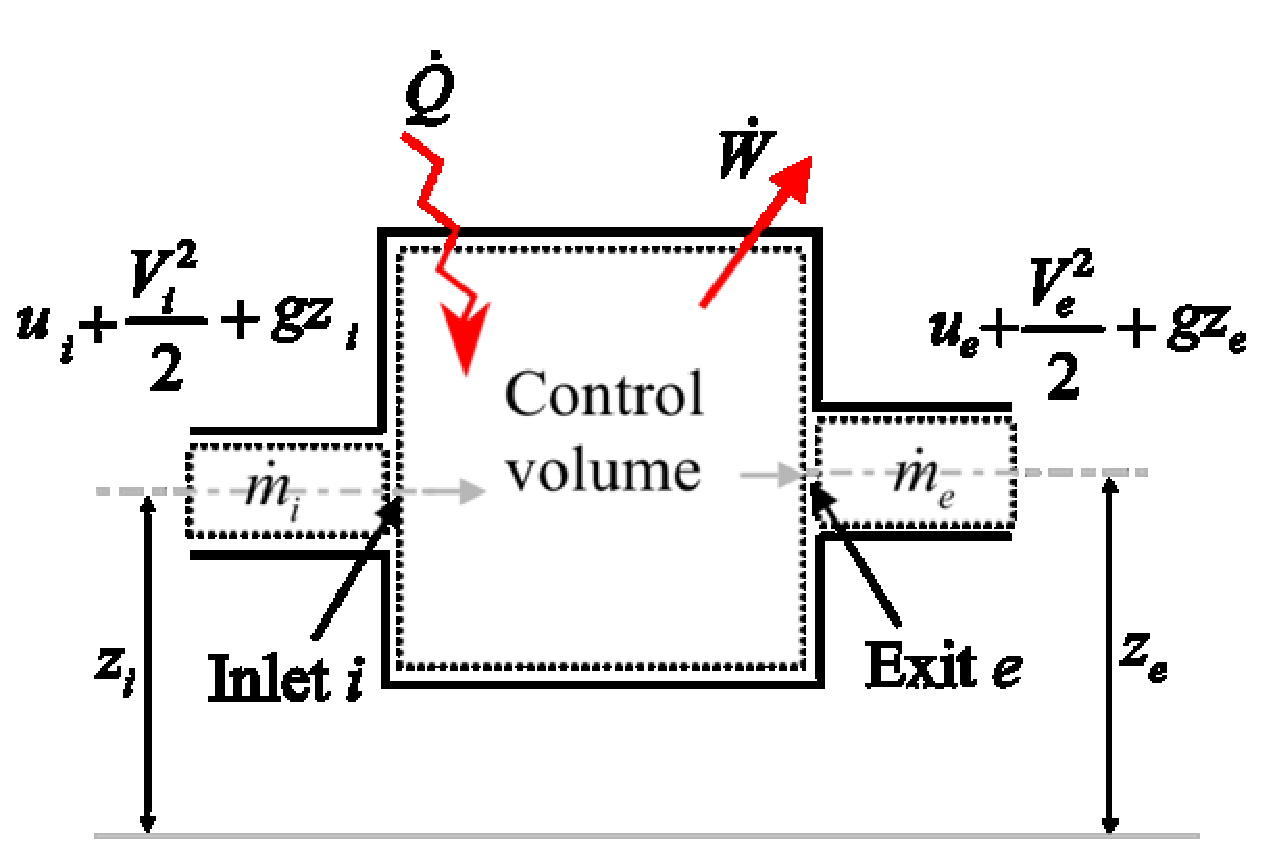
\includegraphics[scale=0.5]{ME21B196/CV.eps}
			}
	\end{center}
	
	\caption{The diagram of a control volume. Credits: \href{https://www.chegg.com/homework-help/fundamentals-of-engineering-thermodynamics-8th-edition-chapter-4-problem-1e-solution-9781118412930}{Chegg.com}.}

	\label{CV}
\end{figure}

\begin{table}[h!]

\begin{center}

	\caption{Key of symbols}
	
	\begin{tabular}{|c|r|l|}

\hline
	Sl No. & Symbol & Explanation \\
	\hline
	1 & $Q$ & Heat interaction of the system \\
	2 & $W$ & Work interaction of the system \\
	3 & $E$ & Total energy of the system \\
	4 & $t$ & Time \\
	5 & $m$ & Mass \\
	6 & $h$ & Specific enthalpy \\
	7 & $g$ & Acceleration due to gravity \\
	8 & $z$ & Height from a reference height \\
	9 & $v$ & Velocity \\
	\hline

\end{tabular}

\end{center}

\end{table}